%--------------------------------------------------------------------------------------
% Dokumentum formátuma
%--------------------------------------------------------------------------------------
\documentclass[12pt]{article}

%--------------------------------------------------------------------------------------
% Változók beállítása
%--------------------------------------------------------------------------------------

%TODO Állítsd be az alábbi változókat

% Szerző
\def\szerzoA {Gyenge Ákos}
\def\szerzoB {Takács Donát}
\def\szerzoC {}
\def\szerzoD {}

% Munka címe
\def\cim {Projektfeladat beszámoló}
\def\alcim {Cubesat tervezése}

\def\hely {Budapest}
\def\datum {\today}


%--------------------------------------------------------------------------------------
% Inicializáció (valószínűleg nem kell hozzányúlni)
%--------------------------------------------------------------------------------------
% Csomagok betöltése

\usepackage[english,magyar]{babel}      % Alapértelmezés szerint utoljára definiált 
% nyelv lesz aktív, de később külön beállítjuk 
% az aktív nyelvet.


%\usepackage{cmap}
\usepackage{amsfonts,amsmath,amssymb}   % Matematikai szimbólumok
\usepackage{graphicx}

\usepackage{geometry}                   % Margók
\usepackage{setspace}                   % Sorköz
\usepackage{booktabs}                   % Jó táblázatok
\usepackage{fancyhdr}                   % Jó élőfejek

\usepackage[unicode]{hyperref}          % Linkek
\usepackage{xcolor}                     % Syntax highlihting
\usepackage{listings}                   % Forráskódokhoz
\usepackage[hang]{caption}              % Jobb képfeliratok
\usepackage[numbers]{natbib}            % Bibliográfia stílus
\usepackage{xspace}                     % Helykihagyás
\usepackage{ifthen}


% Karakterkódolás beállítása (xetex - lualatex és pdflatex külön kezelve)
% http://tex.stackexchange.com/a/47579/71109
\usepackage{ifxetex}
\usepackage{ifluatex}
\newif\ifxetexorluatex % a new conditional starts as false
\ifnum 0\ifxetex 1\fi\ifluatex 1\fi>0
   \xetexorluatextrue
\fi

\ifxetexorluatex
  \usepackage{fontspec}
\else
  \usepackage[T1]{fontenc}
  \usepackage[utf8]{inputenc}
  \usepackage[lighttt]{lmodern}
\fi

% LaTeX és csomagok beállításai

%--------------------------------------------------------------------------------------
% Betűtípus
%--------------------------------------------------------------------------------------
% %ez az alap               % Latin Modern
\usepackage{dejavu}
%\usepackage{kpfonts}        % Palatino Linotype alternatíva
% \usepackage{libertine}    % Times New Roman alternatíva
% egyéb fontok: https://tug.org/FontCatalogue/

%--------------------------------------------------------------------------------------
% Változók
%--------------------------------------------------------------------------------------
\def\szerzok{\szerzoA}

\makeatletter
\ifthenelse{\equal{\szerzoB}{}}{}{\g@addto@macro\szerzok{, \szerzoB}}
\ifthenelse{\equal{\szerzoC}{}}{}{\g@addto@macro\szerzok{, \szerzoC}}
\ifthenelse{\equal{\szerzoD}{}}{}{\g@addto@macro\szerzok{, \szerzoD}}
\makeatother

\author{\szerzok}
\title{\cim}

%--------------------------------------------------------------------------------------
% Oldal layout
%--------------------------------------------------------------------------------------
% we need to redefine the pagestyle plain
% another possibility is to use the body of this command without \fancypagestyle
% and use \pagestyle{fancy} but in that case the special pages
% (like the ToC, the References, and the Chapter pages)remain in plane style

\pagestyle{plain}
\geometry{paper=a4paper}
\geometry{inner=30mm, outer=20mm, top=20mm, bottom=25mm}

\setcounter{tocdepth}{3}
\setcounter{secnumdepth}{3}

%--------------------------------------------------------------------------------------
% Szövegbeállítások
%--------------------------------------------------------------------------------------

\onehalfspacing                 % másfeles sorköz
%\singlespacing					% (egyszeres sorköz)
\selectlanguage{magyar}         % nyelv (magyar.ldf)
\setlength{\parindent}{2em}     % bekezdés behúzás mértéke (magyaros: 2em, angolos: 0)
\setlength{\parskip}{8pt}       % bekezdések közti térköz
\frenchspacing                  % mondatok közt is csak 1 "szóköznyi" kihagyás legyen

% Ha inkább angol beállítások kellenek:
	% \selectlanguage{english}
	% \setlength{\parindent}{0em}
	% \setlength{\parskip}{0.5em}
	% \nonfrenchspacing
	% \renewcommand{\figureautorefname}{Figure}
	% \renewcommand{\tableautorefname}{Table}
	% \renewcommand{\partautorefname}{Part}
	% \renewcommand{\chapterautorefname}{Chapter}
	% \renewcommand{\sectionautorefname}{Section}
	% \renewcommand{\subsectionautorefname}{Section}
	% \renewcommand{\subsubsectionautorefname}{Section}


\sloppy                                 % Margón túllógó sorok tiltása.
\widowpenalty=10000 \clubpenalty=10000  % A fattyú- és árvasorok elkerülése
\def\hyph{-\penalty0\hskip0pt\relax}    % Kötőjeles szavak elválasztásának engedélyezése


%--------------------------------------------------------------------------------------
% Bibliográfia stílusa
%--------------------------------------------------------------------------------------
\bibliographystyle{include/huplain}


%--------------------------------------------------------------------------------------
% Linkek és pdf címkék (hyperref)
%--------------------------------------------------------------------------------------
\hypersetup{
    % bookmarks=true,               % show bookmarks bar?
    unicode=true,                   % non-Latin characters in Acrobat's bookmarks
    pdftitle={\cim},                % title
    pdfauthor={\szerzok},           % author
    pdfsubject={},                  % subject of the document
    pdfcreator={},                  % creator of the document
    pdfproducer={},                 % producer of the document
    pdfkeywords={},                 % list of keywords (separate then by comma)
    pdfnewwindow=true,              % links in new window
    colorlinks=true,                % false: boxed links; true: colored links
    linkcolor=black,                % color of internal links
    citecolor=black,                % color of links to bibliography
    filecolor=black,                % color of file links
    urlcolor=black                  % color of external links
}


%--------------------------------------------------------------------------------------
% listings csomag (forráskód megjelenítés) beállításai
%--------------------------------------------------------------------------------------
\definecolor{lightgray}{rgb}{0.95,0.95,0.95}
\lstset{
	basicstyle=\scriptsize\ttfamily, % print whole listing small
	keywordstyle=\color{black}\bfseries, % bold black keywords
	identifierstyle=, % nothing happens
	% default behavior: comments in italic, to change use
	% commentstyle=\color{green}, % for e.g. green comments
	stringstyle=\scriptsize,
	showstringspaces=false, % no special string spaces
	aboveskip=3pt,
	belowskip=3pt,
	backgroundcolor=\color{lightgray},
	columns=flexible,
	keepspaces=true,
	escapeinside={(*@}{@*)},
	captionpos=b,
	breaklines=true,
	frame=single,
	float=!ht,
	tabsize=2,
	literate=*
		{á}{{\'a}}1	{é}{{\'e}}1	{í}{{\'i}}1	{ó}{{\'o}}1	{ö}{{\"o}}1	{ő}{{\H{o}}}1	{ú}{{\'u}}1	{ü}{{\"u}}1	{ű}{{\H{u}}}1
		{Á}{{\'A}}1	{É}{{\'E}}1	{Í}{{\'I}}1	{Ó}{{\'O}}1	{Ö}{{\"O}}1	{Ő}{{\H{O}}}1	{Ú}{{\'U}}1	{Ü}{{\"U}}1	{Ű}{{\H{U}}}1
}


%--------------------------------------------------------------------------------------
% Saját parancsok
%--------------------------------------------------------------------------------------
\newcommand{\code}[1]{{\upshape\ttfamily\scriptsize\indent #1}}
% A hivatkozások közt így könnyebb DOI-t megadni: \doi{xxxx.yyyy}
\newcommand{\doi}[1]{DOI: \href{http://dx.doi.org/\detokenize{#1}}{\raggedright{\texttt{\detokenize{#1}}}}}

\DeclareMathOperator*{\argmax}{arg\,max}
\DeclareMathOperator{\sign}{sgn}
\DeclareMathOperator{\rot}{rot}

%--------------------------------------------------------------------------------------
% Képaláírás stílusa
%--------------------------------------------------------------------------------------
\captionsetup[figure]{
	width=.75\textwidth,
	aboveskip=10pt}

\renewcommand{\captionlabelfont}{\it}
\renewcommand{\captionfont}{\footnotesize\it}

%--------------------------------------------------------------------------------------
% Elválasztás kivételei
%--------------------------------------------------------------------------------------
\hyphenation{Shakes-peare Mar-seilles ár-víz-tű-rő tü-kör-fú-ró-gép}

%--------------------------------------------------------------------------------------
% Dokumentum törzse
%--------------------------------------------------------------------------------------

\begin{document}
\pagenumbering{arabic}        % Oldalak számozása

% Címoldal
\hypersetup{pageanchor=false}

%--------------------------------------------------------------------------------------
%	Címoldal [Title page]
%--------------------------------------------------------------------------------------
\begin{titlepage}
\begin{center}

\includegraphics[width=60mm]{images/kozmosz-logo}\\
\vspace{0.3cm}

\textbf{BME vagy valami ilyesmi}

\vspace{0.1cm}

Egyéb szöveg amit ide akarsz írni

\vspace{5cm}

{\huge \MakeUppercase{\cim}}\\
\vspace{0.8cm}
{\LARGE \alcim}

\vspace{4cm}

{\large \textit{Készítette}}
\vspace{0.3cm}

{\large
    \szerzoA

    \szerzoB

    \szerzoC

    \szerzoD
}

\vfill
{\LARGE Budapest, \datum}
\end{center}
\end{titlepage}

% Tartalomjegyzék
\tableofcontents\vfill


\section{Az Apollo-program}

Az Apollo-program az Egyesült Államok második – a hosszas előkészítő fázisa miatt a repülések sorrendjét tekintve harmadik – emberek részvételével végrehajtott űrprogramja volt, amely 1961 és 1972 között zajlott. A program célja kettős volt: a fő célként az ember Holdra juttatása fogalmazódott meg, mögöttes politikai célként pedig a hidegháború által életre hívott űrversenyben az USA vesztes pozíciójának megfordítása, a nemzeti presztízs helyreállítása volt a célkitűzés.

A holdprogram hivatalos bejelentése 1961. május 25-én John F. Kennedy elnök kongresszusi beszédében történt, ezt tekintjük az Apollo-program hivatalos kezdetének. A beszédben Kennedy 9 éves határidőt tűzött ki a program megvalósításra. A célt 1969. július 21-én, az Apollo–11 űrhajósainak, Neil Armstrongnak és Buzz Aldrinnak a Holdra lépésével sikerült teljesíteni. Őket még további öt űrhajóspáros követte, így összesen hat sikeres holdra szállást teljesítettek a NASA űrhajósai. Armstrongék holdra szállását négy, űrhajósokkal végrehajtott tesztrepülés előzte meg, míg egy sikertelen holdutazás is része volt a programnak. A repülések mellett egy tragédia is beárnyékolta az Apollo-programot, az első tesztrepülés előtti előkészületek közben három űrhajós, Gus Grissom, Ed White és Roger Chaffee halt meg az űrkabinjukban kitört tűz következtében.

\begin{figure}[htb]
  \centering
  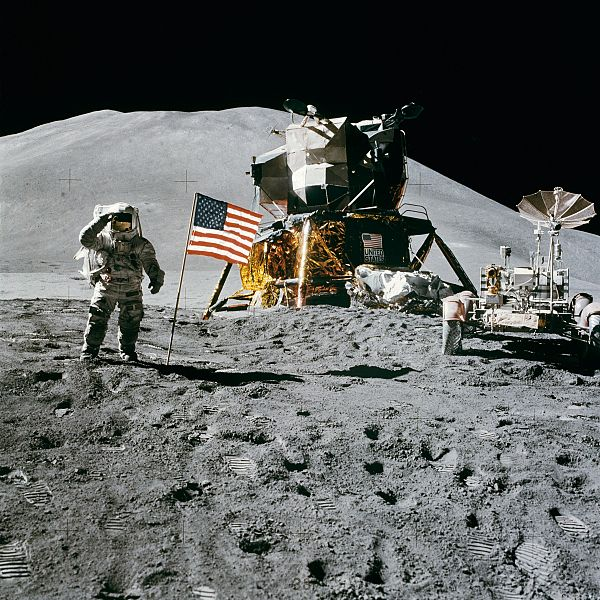
\includegraphics[width=0.5\textwidth]{images/foto}
  \caption{A Hold meghódítása}
  \label{fig:foto}
\end{figure}

A repüléseket egy speciális űrhajórendszerrel hajtották végre, amely az Apollo típusú űrhajóból és a holdra szállás kulcsának számító holdkompból állt, hordozóeszközként pedig szintén speciálisan a feladathoz tervezett Saturn V és Saturn IB rakétákat használtak. A program hardverét később sikerrel alkalmazták más űrkutatási programokban is, így a Skylab-programban és az Szojuz–Apollo repülésen is.

A program 1972-ben fejeződött be, azóta egyetlen embert szállító űrhajó sem hagyta el az alacsony Föld körüli pályát. Az űrhajósok által visszahozott kőzetminták és a kihelyezett műszerek mérései forradalmi változásokat hoztak a Naprendszer történetének, kialakulásának megismerésében, a Föld-Hold rendszer fejlődéstörténetének ismereteiben.

Az Egyesült Államok az Apollo-programra több mint 19,5 milliárd dollárt költött.

\section{Előzmények}

\subsection{Korai elképzelések}

Röviddel Konsztantyin Ciolkovszkij rakétaelvet megalkotó munkáinak publikálása után megjelentek az első elképzelések a világűr, azon belül pedig a legkézenfekvőbb cél, a Hold elérésére. Ezek közül a később legértékesebbnek bizonyult elképzelés Jurij Kondratyuk munkája volt, aki az anyaűrhajó/holdkomp rendszerű holdra szállás elméleti alapjait fektette le. Fantasztikus elképzelésekben később sem volt hiány, ilyen volt a három legkomplexebb ismeretekkel rendelkező tudós, Wernher von Braun rakétamérnök, Fred Whiplle és Willy Ley csillagászok publikációja a Holdutazás megvalósításáról a Colier's magazinban,[5] ami utópiának tűnt az 1950-es évek elején. Ebben az elképzelésben 15 űrhajós utazott volna, három óriási űrhajóval, amelyeket Föld körüli pályán szereltek volna össze, majd töltöttek volna fel üzemanyaggal. A háromból az egyik teherűrhajó lett volna, aminek célja pusztán a visszaútra szükséges üzemanyag szállítása lett volna. A leszállás után 6 hétig lettek volna az űrhajósok a Hold felszínén, napfelkeltétől kezdve egészen a következő – négy földi hétig tartó – nappal végéig. A kiürült üzemanyagtartályok hengereit lakómodulokká lehetett volna alakítani, egyfajta Hold-bázist létrehozva. Az építkezést daruk, és egy tíztonnás traktor (amit a későbbi felfedező utak járműveként is lehetett volna használni) könnyítette volna meg. Ennek az elképzelésnek a megvalósításához több száz tonna anyagot kellett volna megmozgatni, mindezt abban az időben, amikor az 1 tonnás Mercury-űrkabint sem tudták biztonságosan Föld körüli pályára állítani.[6]

\begin{table}[htb]
  \caption{Repülések}
  \centering
  \begin{tabular}{ccc}
    \toprule
    Repülés & Dátum & Időtartam \\
    \midrule
    Apollo-7 & 1968 október 11. & 11 nap \\
    Apollo-8 & 1968 november 21. & 7 nap \\
    Apollo-9 & 1969 március 3 &  10 nap \\
    \bottomrule
  \end{tabular}
  \label{tab:repulesek}
\end{table}

\subsection{Közvetlen előzmények}

\subsubsection{„Szputnyik-krízis”}

A hidegháború két egymással vetekedő nagyhatalma az 1950-es évek végén, a nemzetközi geofizikai év tudományos kísérlet- és rendezvénysorozatában találta meg azt az új területet, ahol kiterjeszthetik a technológiai versengésüket: az Egyesült Államok és a Szovjetunió egyaránt a világűrbe kívánta juttatni a maga űreszközét. A cél a másik fél fölötti technológiai fennhatóság bizonyítása volt. A versenyt a szovjetek nyerték, amikor 1957. október 4-én sikerrel juttatták az űrbe az addig titokban fejlesztett rakétájukkal a Szputnyik–1-et. Az USA-ban ezt szinte háborús hadüzenetként értelmezték (a szovjetek érdemi üzenete a műhold Föld körüli pályára állításával az volt: ha körbe tudunk juttatni a Földön egy tárgyat, akkor a Föld bármely pontját elérhetjük, bármely pontját képesek vagyunk bombázni).

Az USA vezetése elfogadta a szovjet kihívást és koncentrált erőfeszítést tett az űrteljesítmények területén az ellenfél előnyének behozására. E cél elérésére létrehozták a NASA-t, amely az összes korábban létrehozott repülési és űrhajózási kísérleti műhelyt vonta egy szervezetbe, hogy az erőket egyesítve minél hatékonyabban érjék el a kitűzött célt. 


%--------------------------------------------------------------------------------------
% Bibliográfia
%--------------------------------------------------------------------------------------
\addcontentsline{toc}{section}{Irodalomjegyzék}
\bibliography{bibliografia}


%--------------------------------------------------------------------------------------
% Mellékletek
%--------------------------------------------------------------------------------------
\appendix
\addcontentsline{toc}{section}{Mellékletek}

\section{Kapcsolási rajzok}

\section{Röppálya-kalkuláció}



\end{document}
